\documentclass[11pt]{article}

\usepackage[T1]{fontenc}
\usepackage[utf8]{inputenc}
\usepackage{lmodern}
\usepackage[margin=1in]{geometry}
\usepackage{amsmath,amssymb}
\usepackage{booktabs}
\usepackage{graphicx}
\usepackage{xcolor}
\usepackage[round,authoryear]{natbib}
\usepackage[hidelinks]{hyperref}
\usepackage{url}
\usepackage[font=small,labelfont=bf]{caption}
\usepackage{microtype}
\usepackage{enumitem}
\setlist{itemsep=2pt,topsep=4pt}

\newcommand{\dF}{$\Delta$F1}
\newcommand{\repo}{\url{https://github.com/magazine233/knowing-the-graph}}
\newcommand{\devrepo}{\url{https://github.com/magazine233/ARENA_3.0}}

\title{Knowing the Graph: Does Relational Structure Improve\\Linear-Probe Detection of Related AI-Safety Concepts?}
\author{Jason Boudville\\[2pt]
\small Independent; carried out during the TARA program\\[6pt]
\small Second-model results: independent peer replication and extension by \textbf{p0ss} (HatCat)}
\date{}

\begin{document}
\maketitle

\begin{abstract}
AI-safety concepts such as manipulation, deception and sycophancy are related to one another: they form a
graph of siblings and hubs rather than a list of independent categories. We ask whether knowing that graph
improves linear-probe detection of 15 related concepts in the residual stream of Gemma-2-9B, with an independent
peer replication on Gemma-4-E4B. Across four iterations, with every powered test after the first pre-registered,
we find two results. First, relations help as \emph{local hard negatives}: a concept's declared siblings are
more confusable with it than unrelated concepts (\dF{} $+0.055$ across 15 concepts, Wilcoxon
$p=1.5\times10^{-4}$, pre-registered), and training a concept's probe against its direct neighbours improves
discrimination by about $+0.06$ F1 on both models. Exploratory controls suggest roughly a third of the sibling
effect is shared vocabulary. Second, we find no measurable benefit from the graph's \emph{connectivity}. When the
evaluated sibling is withheld from the negatives, the remaining graph structure recovers \dF{} $\approx +0.01$,
and a pre-registered tenfold data-volume sweep does not raise it: at 70 passages per concept per context the
mean is $+0.005$ (95\% CI $[-0.005, +0.014]$), and net of vocabulary overlap it is $-0.006$. This rules out a
connectivity benefit much larger than $+0.015$ F1 on this graph, but not one near our minimum detectable effect
of $0.014$. The test is also limited by the graph itself (15 concepts, 26 edges, at most four alternate paths
per edge), so we scope the null to this graph. We describe a post-hoc account, \emph{independent-constraint
boundary coverage}, that fits both results, and draw a deployment consequence: each negative-selection scheme
seals only the boundary face it trains against. On a pre-specified test with legitimate-influence passages
(negotiation, advertising, lobbying), no scheme reduces false positives, which stay near $0.23$ on held-out
contexts.
\end{abstract}

% =====================================================================================================
\section{Introduction}

Deployable monitoring for AI-safety-relevant behaviour increasingly relies on concept-detection probes: linear
read-outs of a model's internal activations that flag, for example, deception or sycophancy
\citep{alain2016probes,zou2023repe,macdiarmid2024sleeper,goldowskydill2025deception}. Safety concepts rarely come
alone. Manipulation borders persuasion; misinformation and disinformation differ only in intent; sycophancy,
unwarranted praise and excessive agreement form a tight family \citep{carroll2023manipulation,park2024deception,sharma2024sycophancy}.
A monitor needs one detector per concept across a whole family, and the family's structure is often available
for free in an ontology. The obvious hope is that this structure can substitute for data.

We test a specific form of that hope, inherited from the HatCat concept-lens programme \citep{hatcat}. It has two
parts. (H1) Relationship-aware training improves discrimination between related concepts. (H2) The benefit
scales with graph connectivity: if two concepts are joined by many vertex-disjoint paths \citep{menger1927}, a
probe should be able to triangulate their boundary from the surrounding relationships even without direct
evidence about that boundary.

Our answer, after four iterations, is bounded. H1 holds in a narrow form: relations are useful as \emph{hard
negatives}, and the benefit is local to the boundary being tested. H2 finds no support at the data volumes and
graph we could test. We also report where the useful part stops: negatives chosen from the graph do nothing for
legitimate influence that sits just outside the concept family.

The route to this answer is part of the result. Our first iteration produced an apparent positive that did not
survive adversarial checking (Appendix~\ref{app:history}). After it, every powered test was pre-registered with a
locked decision rule, every positive result was checked by an independent refutation pass, and the study was
independently replicated and extended on a second model by p0ss, who originated the hypothesis. The
pre-registration documents and their commit history are public (Appendix~\ref{app:prereg}).

\paragraph{Contributions.}
\begin{enumerate}
  \item A pre-registered test of whether declared relations identify the confusable pairs, with a placebo-graph
        control and an exploratory vocabulary control that together bound the effect (\S\ref{sec:local}).
  \item A pre-registered within-model data-volume sweep of the held-out-edge test, the condition that separates
        graph connectivity from adjacency, with across-edge confidence intervals, a reported minimum detectable
        effect, and a vocabulary-adjusted estimate (\S\ref{sec:connectivity}).
  \item Cross-model agreement: Gemma-2-9B (this work) and Gemma-4-E4B (peer replication) give the same pattern of
        effects on independently generated datasets (\S\ref{sec:local}, \S\ref{sec:connectivity}).
  \item An account of the pattern in terms of independent boundary constraints rather than path counts, stated
        with its limits (\S\ref{sec:account}).
  \item A measured deployment boundary: a rejection test on legitimate influence, pre-specified before it was
        run, in which no negative-selection scheme helps (\S\ref{sec:deploy}).
\end{enumerate}

% =====================================================================================================
\section{Related work}
\label{sec:related}

\paragraph{Probing methodology.} Linear probes read out information that is linearly decodable from a layer
\citep{alain2016probes,kim2018tcav}. Decodability is not the same as use, and a probe can succeed on surface
regularities in the data rather than the intended property \citep{belinkov2022probing}. Control tasks
\citep{hewitt2019control} address this by comparing against a probe's performance on a task it should fail. Our
out-of-distribution context split and vocabulary regressions serve the same purpose: lexical overlap is the
strongest competing explanation for every effect we report.

\paragraph{Concept geometry.} Under the linear representation hypothesis, concepts correspond to directions
\citep{park2024linear}. \citet{park2025hierarchical} extend this to categories and hierarchies, finding that
hierarchically related WordNet concepts occupy orthogonal subspaces in Gemma and LLaMA-3. Our question is
complementary. We take a curated, non-hierarchical graph of safety concepts and ask whether its relations are
\emph{useful for training probes}, not whether they are reflected in geometry. Our geometry check
(\S\ref{sec:account}) finds local adjacency reflected and graded graph distance not. Related work on truth
directions \citep{marks2023truth,burns2023ccs} and representation engineering \citep{zou2023repe} motivates
reading safety-relevant properties linearly. Raw cosine similarity between transformer activations is dominated
by a common direction \citep{ethayarajh2019contextual}, and mean-centring is the standard correction
\citep{mu2018allbutthetop}; we apply it.

\paragraph{Probes for safety-relevant behaviour.} Linear probes have been used to detect strategic deception
\citep{goldowskydill2025deception} and backdoored ``sleeper agent'' behaviour \citep{macdiarmid2024sleeper}. Both
report strong separation and both note that false positives on benign but related inputs are the practical
bottleneck. Our near-out-of-set test (\S\ref{sec:deploy}) measures exactly that failure for a family of
influence concepts.

\paragraph{Hard negatives.} Choosing negatives near the decision boundary is a long-standing technique in metric
and contrastive learning \citep{schroff2015facenet,kalantidis2020mixing,robinson2021hard}. Our positive result
is an instance of it: graph siblings are good hard negatives. The open question we test is whether a graph adds
anything \emph{beyond} supplying nearby negatives.

\paragraph{Rejection.} A classifier without a reject option assigns every input to some class
\citep{chow1970reject,geifman2017selective}. Confidence thresholds are a weak out-of-distribution detector
\citep{hendrycks2017baseline}; training against auxiliary outliers is stronger \citep{hendrycks2019oe}. Our
two-level probe and ``other'' tier (\S\ref{sec:deploy}) are applications of these ideas to concept lenses.

\paragraph{Pre-registration.} Pre-registration separates confirmatory from exploratory analysis
\citep{nosek2018prereg}. We follow that distinction throughout and label every analysis that was not locked in
advance. A null under a ``confidence interval spans zero'' rule is weaker than an equivalence test
\citep{lakens2017equivalence}; we report what our intervals exclude rather than claiming equivalence.

% =====================================================================================================
\section{Setup}
\label{sec:setup}

\paragraph{Concepts.} SET~G is 15 AI-safety concepts from the manipulation, deception and influence family
(Appendix~\ref{app:concepts}), selected from HatCat applied melds layered on the SUMO/WordNet concept pack
\citep{hatcat,niles2001sumo,fellbaum1998wordnet}.

\paragraph{Three graphs.} The study uses three operationalisations of ``related'', and we keep them separate.
(i)~\emph{Ontology graph} (23 edges), derived from HatCat relations and used for the iteration-2 connectivity test
(\S\ref{sec:connectivity}); \texttt{ManipulativeCommunication} is adjacent to 12 of the other 14 concepts, and 84
of the 105 concept pairs have vertex connectivity $k=1$. (ii)~\emph{Declared siblings} (18 pairs), hand-written
discriminating pairs used for the Path-2 hard-negative test (\S\ref{sec:local}). (iii)~\emph{Contrastive boundary
graph} \texttt{SET\_G\_N15\_graph\_contrastive\_boundary\_v1} (26 edges, each with a written rationale and boundary
question), used for the held-out-edge test and the scaling sweep. Its hub is again
\texttt{ManipulativeCommunication}, with degree 7.

\paragraph{Data.} Each concept has a one-sentence definition. Passages were generated by Claude Opus~4.8
\citep{anthropic2026opus48} in four surface-distinct contexts (workplace, online, personal relationships,
marketplace). For the scaling sweep we generated 70 passages per concept per context (4,200 total). A blind audit
asked the same model to assign each passage to one of the 15 concepts from definitions alone: mean self-match was
94.7\%, lowest for the hub concept \texttt{ManipulativeCommunication} (70.4\%). The near-out-of-set controls
(\S\ref{sec:deploy}) are 84 passages for three legitimate-influence concepts, all 84 self-matched under the same
audit.

\paragraph{Probes and evaluation.} We mean-pool the residual stream at layer~18 (Gemma-2-9B, $d=3584$,
\citealp{gemma2024gemma2}; Gemma-4-E4B, $d=2560$, the same block index, \citealp{gemma4e4b}) and fit balanced
logistic-regression probes. Evaluation is always out of distribution: probes are trained on some contexts and
tested on a held-out one. This matters. An early version without the context split saturated at AUC $\approx 1.0$
on surface vocabulary, leaving nothing to measure. F1 is the pre-registered primary metric throughout; balanced
accuracy and AUC give the same ordering in every comparison.

\paragraph{Negative-selection conditions.} For the graph-contrastive test (designed by p0ss) the unit is a
directed edge, target $\rightarrow$ sibling. For each edge, held-out context and seed, we train a target-vs-negatives
probe on the other three contexts and test target versus sibling on the held-out context. Positives and negative
\emph{counts} are identical across conditions; only negative membership changes (Fig.~\ref{fig:conditions}):
\begin{itemize}
  \item \textbf{random}: count-matched non-neighbours of the target (the baseline);
  \item \textbf{direct neighbours}: the target's graph neighbours, including the evaluated sibling;
  \item \textbf{graph-aware mixed}: 40\% direct neighbours, 30\% distance-2, 20\% distant, 10\% same-cluster;
  \item \textbf{held-out edge}: the same graph-aware mix \emph{excluding the evaluated sibling}.
\end{itemize}
The held-out-edge condition is the connectivity test. If the rest of the graph carries information about a
boundary, it should partly reconstruct that boundary when the sibling itself is never seen as a negative. With
26 edges, 2 directions, 4 contexts and 30 seeds there are 6,240 paired comparisons per condition.

\begin{figure}[t]
  \centering
  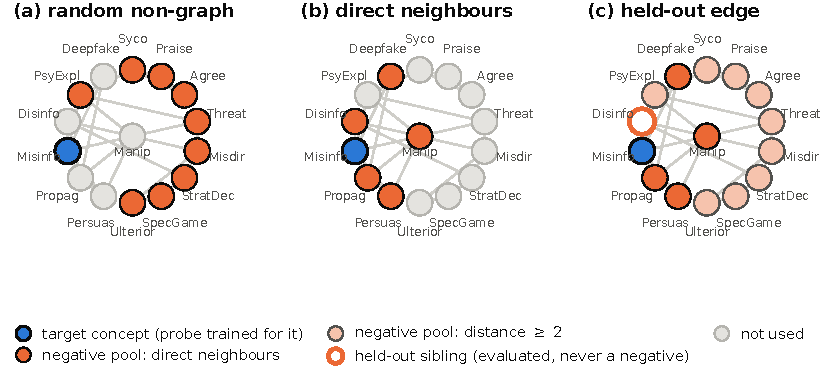
\includegraphics[width=\linewidth]{figures/fig1_conditions.pdf}
  \caption{Negative-selection conditions on the contrastive boundary graph, for one target
  (\texttt{Misinformation}) and one evaluated sibling (\texttt{Disinformation}). Only which concepts serve as
  negatives changes; negative counts are matched. In the held-out-edge condition the evaluated sibling is never
  a negative, so any benefit must come from the rest of the graph. The graph-aware mixed condition (not shown)
  is panel (c) with the sibling included.}
  \label{fig:conditions}
\end{figure}

\paragraph{Statistics.} We average the 120 comparisons for each directed edge (4 contexts $\times$ 30 seeds) to a
single per-edge value and test the 52 per-edge means against zero (one-sample $t$, with Wilcoxon as a
distribution-free check). Seeds share data, so testing all 6,240 comparisons would overstate precision. Edges
also share endpoints, so even the per-edge intervals are somewhat optimistic; we return to this in
\S\ref{sec:limits}. The minimum detectable effect (MDE) is computed at 80\% power, two-sided $\alpha=0.05$, from
the observed per-edge spread.

% =====================================================================================================
\section{Relations help as local hard negatives}
\label{sec:local}

\paragraph{Declared siblings are the confusable pairs (pre-registered).} Iterations 1 and 2 had treated
``knowing the relations'' as extra \emph{positive} passages along the graph, and found nothing
(Appendix~\ref{app:history}). p0ss pointed out that the hypothesis's mechanism instead uses related concepts as
\emph{negatives}. We pre-registered the prerequisite test (locked before any probe was trained). For each concept,
a binary out-of-distribution probe separates it from each declared sibling and from each non-sibling, and
$\Delta(C)$ is the F1 gap. Siblings are harder to separate for 13 of 15 concepts (Fig.~\ref{fig:path2}): mean
$\Delta = +0.055$ (F1 0.916 against siblings, 0.971 against non-siblings), Wilcoxon $p = 1.5\times 10^{-4}$, and
$+0.057$ ($p=3\times10^{-4}$) excluding the hub concept.

\paragraph{Two exploratory controls.} Neither was pre-registered; both were added in response to adversarial
review. (a)~\emph{Placebo graphs}: permuting concept labels while preserving graph topology (2,000 permutations)
gives a null distribution centred on zero; the declared graph's sibling gap sits at $z=2.99$, $p=0.002$. The
effect belongs to these particular relations, not to having \emph{a} graph. (b)~\emph{Vocabulary}: declared
siblings share more words (mean Jaccard 0.197 vs.\ 0.179), and word overlap strongly predicts confusability
across all 105 pairs (Spearman $-0.73$). Regressing pair F1 on sibling status and overlap shrinks the sibling
coefficient from the raw gap of 0.049 to 0.031 ($p=4\times10^{-4}$), so about a third of the effect is
attributable to vocabulary. This is an upper bound on the lexical share, because vocabulary partly carries
relatedness. The rank-based version of the same control is marginal (partial Spearman $-0.18$, $p=0.07$).

\begin{figure}[t]
  \centering
  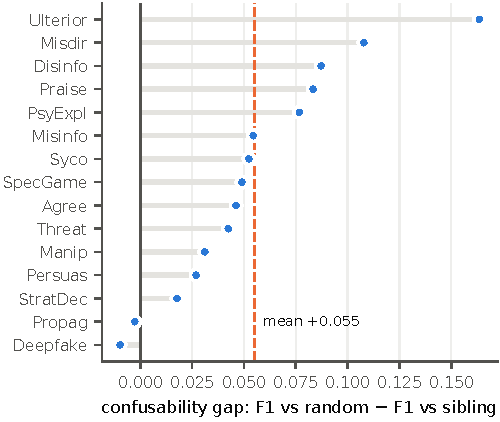
\includegraphics[width=0.62\linewidth]{figures/fig2_path2_confusability.pdf}
  \caption{Declared siblings are more confusable than non-siblings (pre-registered Path-2 test, Gemma-2-9B,
  layer 18, 30 seeds). Each point is one concept's F1 gap between separating it from random non-siblings and
  from its declared siblings. Mean $+0.055$, Wilcoxon $p=1.5\times10^{-4}$. An exploratory placebo test
  (2,000 topology-preserving label permutations) places the declared graph at $z=2.99$, $p=0.002$.}
  \label{fig:path2}
\end{figure}

\paragraph{Training with neighbours as negatives helps, on two models.} The graph-contrastive test
(Table~\ref{tab:contrastive}) turns confusability into a training benefit. On Gemma-4-E4B at 7 passages per
context, the peer replication found direct-neighbour negatives improve F1 by $+0.057$ over count-matched random
negatives, graph-aware mixed negatives by $+0.043$, and held-out-edge negatives by $+0.008$. On Gemma-2-9B at 14
passages per context, with our own independently generated data and the same harness, we obtain $+0.059$,
$+0.039$ and $+0.012$. The two models agree to within 0.004 on every condition. A layer sweep on Gemma-4-E4B
(10 seeds) gives the same ordering at layers 8, 18, 24 and 42. Discrimination is near ceiling at every layer
(concept-versus-neighbour AUC 0.96--1.00 from the embedding layer up), so layer 18 is representative, not
selected.

\begin{table}[t]
  \centering
  \small
  \caption{Graph-contrastive test: mean \dF{} over count-matched random negatives (all 6,240 paired comparisons
  per condition unless noted). E4B rows are the peer replication. Volume is passages per concept per context.}
  \label{tab:contrastive}
  \begin{tabular}{lllrrr}
    \toprule
    Model & Volume & Layer & Direct neighbours & Graph-aware mixed & Held-out edge \\
    \midrule
    Gemma-4-E4B & 7  & 18 & $+0.057$ & $+0.043$ & $+0.008$ \\
    Gemma-4-E4B & 28 & 18 & $+0.055$ & $+0.041$ & $+0.010$ \\
    Gemma-2-9B  & 14 & 18 & $+0.059$ & $+0.039$ & $+0.012$ \\
    Gemma-2-9B  & 70 & 18 & $+0.040$ & $+0.030$ & $+0.005$ \\
    \midrule
    \multicolumn{6}{l}{\emph{Layer sweep, Gemma-4-E4B, 7/context, 10 seeds}} \\
    Gemma-4-E4B & 7 & 8  & $+0.072$ & $+0.045$ & $+0.008$ \\
    Gemma-4-E4B & 7 & 18 & $+0.055$ & $+0.044$ & $+0.008$ \\
    Gemma-4-E4B & 7 & 24 & $+0.066$ & $+0.044$ & $+0.003$ \\
    Gemma-4-E4B & 7 & 42 & $+0.059$ & $+0.043$ & $+0.011$ \\
    \bottomrule
  \end{tabular}
\end{table}

The ordering, direct $>$ mixed $>$ held-out edge, follows how close the negatives are to the boundary being
tested. Once the sibling itself is removed, most of the gain disappears.

% =====================================================================================================
\section{Graph connectivity adds no measurable benefit}
\label{sec:connectivity}

\subsection{Pairwise connectivity test (iteration 2, pre-registered)}
Iteration 2 tested H2 directly on the ontology graph. For all 105 pairs, a volume-matched comparison measured
the out-of-distribution gain from swapping pair-specific boundary passages into the training data, and the
pre-registered primary endpoint was the partial Spearman correlation between gain and $k(A,B)$, controlling for
baseline accuracy. The result was $\rho = -0.125$ ($p=0.20$): no positive relationship. The test had a structural
weakness: 84 of the 105 pairs have $k=1$, and most pairs with $k\ge 3$ involve the hub, so the predictor had little
spread. The test also used relations as extra positives, which \S\ref{sec:local} suggests is the wrong mechanism.
We therefore read it as consistent with, not strong evidence for, the null below.

\subsection{Held-out-edge scaling sweep (iteration 4, pre-registered)}
The held-out-edge condition sat near $+0.01$ on both models at their base volumes (Table~\ref{tab:contrastive}).
The obvious objection is power: perhaps a connectivity signal exists but needs more data. We pre-registered a
within-model sweep to test this. The design was Gemma-2-9B; volumes of 7, 14, 28, 56 and 70 passages per concept
per context, each subsampled from a single 70-per-context generation and extraction; 30 seeds; held-out-edge
\dF{} as the primary endpoint. The locked decision rule was \textsc{confirm} if the delta rises monotonically with
volume and is significantly positive at the top volume, and \textsc{null} if the top-volume confidence interval
spans zero.

\begin{figure}[t]
  \centering
  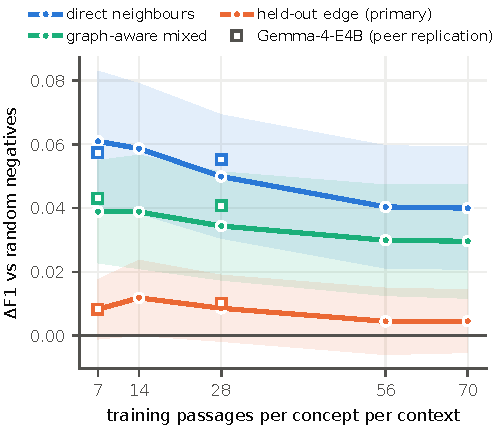
\includegraphics[width=0.6\linewidth]{figures/fig3_scaling_sweep.pdf}
  \caption{Held-out-edge \dF{} (the pre-registered primary, orange) does not rise with data volume. Lines and
  bands: Gemma-2-9B means with 95\% confidence intervals across the 52 directed edges. Hollow squares:
  Gemma-4-E4B from the peer replication, shown as independent corroboration only; the pre-registered trend is
  within-model (Gemma-2-9B). Direct-neighbour and mixed conditions are pre-declared secondary outcomes.}
  \label{fig:sweep}
\end{figure}

\begin{table}[t]
  \centering
  \small
  \caption{Scaling sweep, Gemma-2-9B: across-edge paired tests (52 directed edges, each averaged over 4 contexts
  $\times$ 30 seeds). $p$ is the one-sample $t$-test; MDE is the minimum detectable effect at 80\% power.}
  \label{tab:sweep}
  \begin{tabular}{rrrrrr}
    \toprule
    & \multicolumn{4}{c}{Held-out edge (primary)} & Direct neighbours \\
    \cmidrule(lr){2-5}\cmidrule(lr){6-6}
    Volume & \dF{} & 95\% CI & $p$ & MDE & \dF{} [95\% CI] \\
    \midrule
    7  & $+0.008$ & $[-0.001, +0.018]$ & 0.081 & 0.013 & $+0.061$ $[+0.039, +0.083]$ \\
    14 & $+0.012$ & $[+0.000, +0.024]$ & 0.049 & 0.017 & $+0.059$ $[+0.038, +0.079]$ \\
    28 & $+0.009$ & $[-0.002, +0.019]$ & 0.103 & 0.015 & $+0.050$ $[+0.031, +0.069]$ \\
    56 & $+0.004$ & $[-0.006, +0.015]$ & 0.39  & 0.015 & $+0.040$ $[+0.021, +0.060]$ \\
    70 & $+0.005$ & $[-0.005, +0.014]$ & 0.36  & 0.014 & $+0.040$ $[+0.021, +0.059]$ \\
    \bottomrule
  \end{tabular}
\end{table}

\paragraph{Result.} Held-out-edge \dF{} by volume was $+0.008$, $+0.012$, $+0.009$, $+0.004$, $+0.005$
(Fig.~\ref{fig:sweep}, Table~\ref{tab:sweep}). It does not rise; if anything it falls after 14 per context. At
the top volume the mean is $+0.0046$ with 95\% CI $[-0.0053, +0.0144]$ ($t$-test $p=0.36$, Wilcoxon $p=0.78$).
The interval spans zero, so the pre-registered verdict is \textsc{null}. Held-out-edge negatives beat random
negatives in only 40\% of the 6,240 paired comparisons.

\paragraph{What the null does and does not exclude.} The top-volume interval excludes a mean connectivity benefit
above about $+0.015$ F1 on this graph. It does not exclude a benefit near the MDE of $0.014$, because the upper
bound and the MDE are essentially equal. Since edges share endpoints, the true interval is probably somewhat
wider. We therefore do not claim the connectivity effect is zero, only that it is too small to matter at the
volumes we tested and that more data did not make it larger. The same instrument, at the same volume, clearly
detects the direct-neighbour effect ($+0.040$, CI $[+0.021, +0.059]$, $p=10^{-4}$). One volume deserves mention:
at 14 per context the held-out-edge interval just touches zero ($p=0.049$). This was not the pre-registered
endpoint, is uncorrected across five volumes, and is followed by smaller estimates at every higher volume.

\paragraph{Net of vocabulary.} The pre-registration called for reading the result net of lexical overlap but did
not fix the model; the specification below was chosen after the primary result was known. For each comparison we
compute how much more word overlap (Jaccard) the held-out-edge negatives share with the evaluated sibling than the
random negatives do, average to one value per edge, and regress per-edge \dF{} on it. Vocabulary advantage
strongly predicts the per-edge benefit (slope $+1.72$, $p<0.001$, $R^2=0.32$; Fig.~\ref{fig:peredge}a). The
intercept, the held-out-edge effect at zero vocabulary advantage, is $-0.006$ $[-0.016, +0.003]$. The small
positive gross effect is therefore plausibly lexical.

\paragraph{Per-edge connectivity (exploratory).} The pre-registered endpoint concerns the mean. A direct test of
H2 asks whether edges with \emph{more} alternate routes benefit more. On the contrastive graph, after removing
each edge, its endpoints have between 0 and 4 vertex-disjoint alternate paths (counts 1, 10, 9, 5, 1). Per-edge
held-out-edge \dF{} does not increase with this count (Spearman $\rho=-0.34$, $p=0.085$, 26 edges;
Fig.~\ref{fig:peredge}b). The trend is, if anything, in the wrong direction.

\paragraph{Secondary: the neighbour premium shrinks with data.} Direct-neighbour negatives stay clearly positive at
every volume, but their advantage falls from $+0.061$ to $+0.040$ as volume grows tenfold. Absolute F1 improves in
every condition with more data, and random negatives gain most. Smart negative selection is worth most when data
is scarce, which is the usual situation for long-tail safety concepts.

\subsection{What this test can and cannot show}
\label{sec:scope}
We want to be plain about the reach of the connectivity null. The graph is small: 15 concepts and 26 edges. After
removing an edge, 11 of the 26 have at most one alternate path and none has more than four, so the range of
connectivity being tested is narrow. The earlier pairwise test was narrower still, with 84 of 105 pairs at
$k=1$. The graph was curated by hand, and the result is conditional on it being a sound description of how these
concepts relate. Probe discrimination is near ceiling (random-negative F1 0.92 at the top volume), which
compresses every effect. A graph with many more concepts, genuinely independent alternate paths and harder
boundaries could behave differently. What we can say is that, for a realistic safety-concept family of the size a
practitioner might curate, the graph's connectivity added nothing we could measure beyond what direct neighbours
already provide.

% =====================================================================================================
\section{An account: independent-constraint boundary coverage}
\label{sec:account}

The following account was proposed by p0ss after iteration 3. It is post hoc and we present it as an
interpretation that fits the results, not as a tested theory.

Treat a concept as a centroid with a class-conditional spread, and a probe's decision boundary as lying where that
spread thins. Positive examples mainly sharpen the centroid. Negative examples place \emph{facets} of the
boundary, each mainly on the side that faces the negative. On this picture: extra positives along the graph do
little once the centroid is well estimated (iterations 1--2); a sibling negative moves the facet facing that
sibling (\S\ref{sec:local}); the benefit is ordered by how directly the negatives face the tested boundary (direct
$>$ mixed $>$ held-out); and other relations only help with a withheld boundary if they supply constraints oriented
along it. A path count is a reasonable proxy for ``number of independent constraints'' only when graph edges
correspond to independent directions in representation space. Our evidence suggests they do not here. The
held-out-edge benefit tracks shared vocabulary, not alternate-path count (Fig.~\ref{fig:peredge}). The model's
actual confusions concentrate on the hub (below). On the contrastive graph, however, only 3 of the 19 edges not
touching the hub have every alternate path running through it, so ``alternate paths route through one hub'' is
not literally true of the graph. The claim is about representational correlation, and we have not measured that
directly.

\paragraph{Geometry is consistent (peer replication, Gemma-4-E4B).} Raw cosine similarity suggests every concept
overlaps every other (adjacent pairs 0.971, non-adjacent 0.961), but random passage pairs already sit at 0.892:
the common-direction effect \citep{ethayarajh2019contextual}. After mean-centring, adjacent pairs separate from
non-adjacent ones by $+0.166$ and far-domain controls fall well outside the family ($-0.147$), but graph distance
correlates only weakly with centroid similarity ($r=-0.30$ at layer 18; $-0.27$ to $-0.39$, median $-0.34$, across
all 43 layer positions). Local adjacency is visible in the geometry; graded multi-hop structure is not. Probe
results are unaffected by the correction, since a linear classifier can absorb a common offset.

\paragraph{A forward-looking implication.} The account implies that a boundary face nothing has been trained
against should leak whichever scheme is used. We had already pre-specified a test of one such face before running
it (\S\ref{sec:deploy}). The test was designed as a rejection test, not as a test of the account, so we count it
as consistent with the account rather than as a confirmed prediction.

% =====================================================================================================
\section{Deployment consequences: rejection and tiered negatives}
\label{sec:deploy}

The analyses in this section move from pairwise discrimination to per-concept one-vs-rest lenses evaluated at a
fixed operating point: false-positive rate (FPR) at 95\% true-positive rate, with negative count matched to each
concept's graph degree. Pairwise AUC is near ceiling, but FPR at high recall is sensitive to exactly the boundary
placement that negatives control.

\paragraph{A flat probe cannot say ``none of these'' (peer replication, Gemma-4-E4B).} A 15-way argmax assigns every
far-domain input (passages about dogs, weather, basketball, photosynthesis) to some concept. A confidence threshold
rejects only 26\% of them at 95\% in-family retention (AUROC 0.836). Adding a coarse \emph{other} class trained on
far-domain controls rejects them at recall 1.0, including a held-out far concept it never trained on, with no
false rejection of in-family passages. Hierarchical \emph{classification} is not the fix: flat accuracy 0.910
exceeds soft (0.857) and hard (0.850) coarse-to-fine decoding. The coarse stage is useful for rejection, while
resolution is best left to the flat lens.

\paragraph{Each scheme seals the face it trains against.} Table~\ref{tab:faces} reports FPR by boundary face on
both models. On Gemma-4-E4B, graph-sibling negatives cut neighbour-face FPR from 0.192 to 0.046 but are no better
than random on off-graph confusers (0.257 vs.\ 0.270). Negatives mined from the model's own confusions cut the
off-graph face to 0.058, a 20-point reduction, but give back most of the neighbour gain. A cheap far-domain
\emph{other} tier seals the far face entirely (0.000). We reproduce the structure on Gemma-2-9B (our run, layer 18):
siblings seal neighbours (0.318 $\rightarrow$ 0.032), and mining seals the off-graph face (0.335 $\rightarrow$
0.119). The absolute values differ, the pattern does not. Off-graph confusions matter because the graph misses
the model's hub-attractor errors: in the peer replication, 24 of the flat probe's 42 misclassifications fall on
concept pairs with no edge (a small base; the pattern, not the exact count, is the robust finding). Several
concepts are confused \emph{into} the hub without an edge to it.

\begin{table}[t]
  \centering
  \small
  \caption{False-positive rate at a 95\%-TPR operating point (E4B: 93\% achieved) by boundary face and negative
  scheme, with negative counts matched. Gemma-4-E4B is the peer replication (layer 18). Gemma-2-9B is this work
  (layer 18, 14 lenses, \texttt{PersuasiveCommunication} quarantined); the multi-scale scheme was not run there
  because only one far-domain control set was available. Near-OOS: legitimate-influence passages, pooled and on
  contexts held out of the lens's training fold.}
  \label{tab:faces}
  \setlength{\tabcolsep}{5pt}
  \begin{tabular}{llrrrrr}
    \toprule
    & & & & & \multicolumn{2}{c}{Near-OOS} \\
    \cmidrule(lr){6-7}
    Model & Negatives & Neighbours & Off-graph & Far-OOD & pooled & held-out ctx \\
    \midrule
    Gemma-4-E4B & random        & 0.192 & 0.270 & 0.179 & -- & -- \\
                & graph-sibling & 0.046 & 0.257 & 0.189 & -- & -- \\
                & model-mined   & 0.157 & 0.058 & 0.241 & -- & -- \\
                & multi-scale$^{a}$ & 0.146 & 0.069 & 0.000 & -- & -- \\
    \midrule
    Gemma-2-9B  & random        & 0.318 & 0.335 & n/a$^{b}$ & 0.164 & 0.229 \\
                & graph-sibling & 0.032 & 0.378 & n/a$^{b}$ & 0.175 & 0.225 \\
                & model-mined   & 0.158 & 0.119 & n/a$^{b}$ & 0.182 & 0.227 \\
    \bottomrule
  \end{tabular}\\[3pt]
  \parbox{\linewidth}{\raggedright\footnotesize $^{a}$ model-mined negatives plus the far-domain \emph{other} controls.
  $^{b}$ far-domain set used for evaluation only (nothing trained against it).}
\end{table}

\paragraph{Calibration drift.} In the peer replication, an earlier run that set thresholds on training positives
rather than held-out ones achieved only 34\% held-out TPR (reported in the replication write-up; no result file
was committed for that run). On Gemma-2-9B we measure the same effect more mildly: train-calibrated thresholds
give held-out TPR of 0.75--0.81 instead of 0.95. Lens scores shift across contexts, and a deployed monitor has no
held-out labels with which to notice.

\paragraph{The hard regime: legitimate influence (pre-specified).} Far-domain inputs are the easy rejection case.
The hard case is legitimate influence adjacent to the family: honest negotiation, transparent advertising and
declared lobbying. We generated and audited 84 such passages (3 concepts $\times$ 4 contexts $\times$ 7) and
specified the analysis before running it: score the 14 lenses other than \texttt{PersuasiveCommunication}, which is
quarantined because its own training data includes honest advertising, so firing there is a true positive by
construction; report FPR pooled and split by whether the passage's context was held out of the scoring lens's
training fold.

\begin{figure}[t]
  \centering
  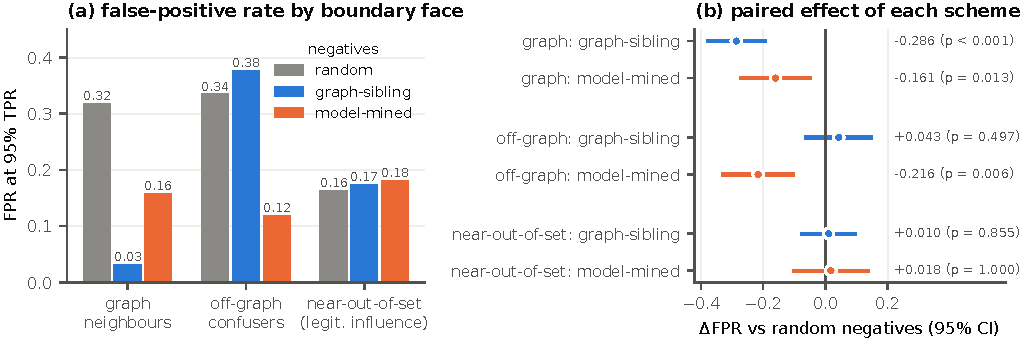
\includegraphics[width=\linewidth]{figures/fig4_near_oos_rejection.pdf}
  \caption{No negative scheme reduces false positives on legitimate influence (Gemma-2-9B, layer 18, 14 lenses).
  (a)~FPR at 95\% TPR by boundary face. Graph-sibling negatives seal the neighbour face and model-mined negatives
  the off-graph face; the near-out-of-set face, trained against by neither, stays flat. (b)~Paired change in FPR
  relative to random negatives across lenses (95\% CI; Wilcoxon $p$). Both positive controls clear zero; both
  near-out-of-set intervals include it. Off-graph tests use the 13 lenses with off-graph confusers.}
  \label{fig:nearoos}
\end{figure}

No scheme reduces the leak (Fig.~\ref{fig:nearoos}). Pooled FPR is 0.164, 0.175 and 0.182 under random,
graph-sibling and model-mined negatives. Paired across the 14 lenses, graph-sibling negatives change it by
$+0.010$ (95\% CI $[-0.074, +0.095]$, Wilcoxon $p=0.86$) and model-mined negatives by $+0.018$ ($[-0.101, +0.136]$,
$p=1.00$). The same lenses and test detect the neighbour seal ($-0.286$, $p<0.001$) and the off-graph seal
($-0.216$, $p=0.006$), so an effect of comparable size here would have been visible. Leakage is significantly
worse on contexts held out of the lens's training fold ($+0.068$, $p=0.016$): the realistic figure is about
$0.23$, roughly one legitimate-influence passage in four, rather than the pooled $0.16$. The leak is concentrated.
Under graph-sibling negatives, \texttt{UnwarrantedPraise} (0.589) and \texttt{ExcessiveAgreement} (0.497) account
for most of it, and three lenses never fire. Honest advertising reads as unwarranted praise and cooperative
negotiation as excessive agreement. The quarantined \texttt{PersuasiveCommunication} lens fires at 0.24--0.52,
well above every scored lens, as expected.

\paragraph{Practical reading.} Cheap tiers (graph siblings plus a far-domain \emph{other} class) seal the
neighbour and far faces; a cheap audit of the model's confusions locates the off-graph gap, where mined negatives
are worth their cost. None of this addresses legitimate influence adjacent to the family, which a deployed monitor
is likely to meet more often than either far-domain text or textbook manipulation. Until that face is trained
against explicitly, practitioners should expect a monitor built this way to fire on roughly one honest-influence
input in four, mostly through a small number of identifiable lenses.

% =====================================================================================================
\section{Limitations}
\label{sec:limits}

\begin{itemize}
  \item \textbf{Scope of the connectivity null.} One small, hand-curated graph with a narrow range of alternate-path
        counts (\S\ref{sec:scope}). The null is conditional on that graph and does not license a general claim
        that concept-graph connectivity is useless for probes.
  \item \textbf{What the interval excludes.} The decision rule (``CI spans zero'') is weaker than an equivalence
        test. The top-volume upper bound ($+0.0144$) is approximately the MDE, so effects near $0.014$ are not
        excluded. Edges share endpoints and are not independent; a concept-level resampling would likely widen
        the interval.
  \item \textbf{Synthetic data, same-model audit.} All passages were written by one model, and the blind audit
        used the same model. Generator-specific phrasing could create or mask effects, and the audit cannot
        detect errors the generator and auditor share. The hub concept self-matched at only 70\%. We have no
        human-written evaluation set.
  \item \textbf{Lexical confounding.} Vocabulary explains a substantial share of every effect we can test for it.
        The out-of-distribution context split reduces but does not remove surface cues.
  \item \textbf{Near ceiling.} Pairwise discrimination is near ceiling on both models, which compresses all deltas;
        the operating-point FPR analysis is the more sensitive instrument.
  \item \textbf{Seed variance understates data variance.} Seeds vary probe training and subsampling, not the
        generated corpus. A fresh generation is a larger source of variation than our intervals reflect, though the
        cross-model agreement on independently generated data is partial reassurance.
  \item \textbf{Exploratory analyses.} The placebo-graph and Path-2 vocabulary controls, the specification of the
        iteration-4 vocabulary control, and the per-edge connectivity test were not pre-registered.
  \item \textbf{Probe and model coverage.} Linear probes at one layer (with an MLP spot-check and an E4B layer sweep),
        mean pooling, two base models, one concept family.
  \item \textbf{Near-out-of-set sample.} 84 passages across three concepts. Adequate for the pooled null, given the
        positive controls; too small to rank which kind of legitimate influence leaks most (per-concept FPRs
        0.155--0.190 under graph-sibling negatives are within noise).
  \item \textbf{Pre-registration record.} The public release repository is a single snapshot. Lock dates are
        verifiable from the commit history of the development repository (Appendix~\ref{app:prereg}).
\end{itemize}

\paragraph{Future work.} The most direct follow-up is to train lenses against near-out-of-set negatives and test
whether that seals the legitimate-influence face without reopening the others. A connectivity retest should use a
larger graph with independently motivated alternate paths, and count representationally independent constraints
rather than vertex-disjoint paths. Contrast-prompted generation (``write A in a way that is not B''; generation
mode alone made no difference, Appendix~\ref{app:generation}), human-written
evaluation data, and sparse-autoencoder features \citep{lieberum2024gemmascope} are natural extensions.

% =====================================================================================================
\section{Conclusion}

For linear probes over a family of related AI-safety concepts, relational structure is useful in a narrow way.
Direct relations make good, cheap hard negatives: about $+0.06$ F1 on two models, perhaps a third of it shared
vocabulary. Beyond that, we found no measurable benefit from the graph's connectivity. A tenfold increase in data
did not raise it, and what little there was tracks vocabulary rather than alternate paths. The negative schemes
we tested seal only the boundary faces they train against, and none of them addresses legitimate influence
adjacent to the family, which leaks at about one passage in four. We think the most useful role for a concept
graph in this setting is as a guide to which negatives to collect, not as a source of structure a probe can
exploit.

% =====================================================================================================
\section*{Contributions and acknowledgements}
J.B. designed and ran iterations 1--4, the Path-2 test, the scaling sweep, the near-out-of-set controls and
rejection test, and wrote the paper. p0ss (HatCat) performed the independent peer replication on Gemma-4-E4B and
contributed the hard-negative reframing, the graph-contrastive test design and contrastive boundary graph, the layer
sweep and anisotropy control, the two-level probe, the multi-scale and confuser-coverage analyses, and the
boundary-coverage account. At p0ss's request their work is credited as a peer replication rather than
co-authorship. The work was carried out as a capstone in the TARA program, which follows the ARENA curriculum
\citep{arena}; no ARENA course code is used. Compute was provided through TARA.

\paragraph{Use of language models.} All passages were generated, and blind-audited, by Claude Opus~4.8.
AI coding and writing assistants were used for analysis code, adversarial review of results, and drafting and
editing this manuscript; all numbers were checked against committed result files.

\paragraph{Code and data availability.} Code, generated passages, audit files, result JSONs and figure scripts:
\repo{} (MIT licence; see its \texttt{NOTICE} for third-party terms). Model weights and raw activations are not
redistributed. Figures in this paper are regenerated by \texttt{paper/figures/make\_figures.py} from committed
JSONs.

\bibliographystyle{plainnat}
\bibliography{references}

% =====================================================================================================
\appendix

\section{Study history}
\label{app:history}
\begin{description}
  \item[Iteration 1.] Definition-only versus relation-augmented multiclass probes, with a correlation between
        per-pair gain and vertex connectivity. An apparent positive at 8 concepts did not replicate at 15, and
        once data volume was matched there was no robust benefit. In hindsight the design also compared conditions
        on different test distributions and treated relations as extra positive passages.
  \item[Iteration 2.] The pre-registered pairwise test in \S\ref{sec:connectivity} (105 pairs, partial Spearman
        $-0.125$, $p=0.20$). A pilot positive at smaller scale was noise.
  \item[Iteration 3 (Path 2).] The reframing to relations as hard negatives and the pre-registered
        confusability test in \S\ref{sec:local}; the graph-contrastive test by the peer replication.
  \item[Iteration 4.] The pre-registered scaling sweep in \S\ref{sec:connectivity}, followed by the pre-specified
        near-out-of-set rejection test in \S\ref{sec:deploy}.
\end{description}

\section{Pre-registration record}
\label{app:prereg}
Lock and result commits in the public development repository \devrepo{} (files under
\texttt{project/capstone/}; branch \texttt{iteration-3}, merged to \texttt{main}). Dates are 2026, times AEST
(UTC+10).

\begin{table}[h]
  \centering
  \small
  \setlength{\tabcolsep}{4pt}
  \begin{tabular}{lllll}
    \toprule
    Test & Locked & Result & Primary endpoint & Outcome \\
    \midrule
    Iteration 2 & \texttt{29c70550} (06-06 11:24) & \texttt{d69f04bd} (06-06 19:10) & partial Spearman, gain vs $k$ & null \\
    Path 2      & \texttt{e927b969} (06-09 13:37) & \texttt{1a91a262} (06-09 14:20) & mean $\Delta(C)>0$ & confirmed \\
    Iteration 4 & \texttt{21c0bf1e} (06-10 07:27) & \texttt{b45eb6c4} (06-12 11:11) & held-out-edge \dF{} & null \\
    Near-OOS    & \texttt{58a54d16} (06-11 21:51) & \texttt{08c84d6d} (08-05 11:05) & FPR, 14 lenses & no effect \\
    \bottomrule
  \end{tabular}
\end{table}

The near-out-of-set analysis was specified in the iteration-4 run book and paper draft rather than in a
standalone pre-registration document. The Path-2 placebo and vocabulary controls were committed with the Path-2
result (\texttt{1a91a262}) and are marked exploratory in their result files.

\section{Generation mode (peer replication)}
\label{app:generation}
p0ss also tested whether activations recorded while Gemma-4-E4B \emph{generates} a concept differ usefully from
activations recorded while it \emph{reads}. Using 420 definition-prompted self-generations, probes built on
autoregressive states and on teacher-forced re-reads of the same tokens passed a check suite (F1, balanced
accuracy and AUC all $\ge 0.80$) at the same rate (0.692 vs.\ 0.693). Reading the generated passage without its
prompt dropped the rate to 0.454, which reflects losing the definition in the prompt rather than a generation
effect. The graph-contrastive ordering (direct $>$ mixed $>$ held-out edge, the last at $+0.002$ to $+0.011$)
holds in every mode. Contrast-prompted generation was not tested.

\section{Per-edge diagnostics}
\label{app:peredge}

\begin{figure}[h]
  \centering
  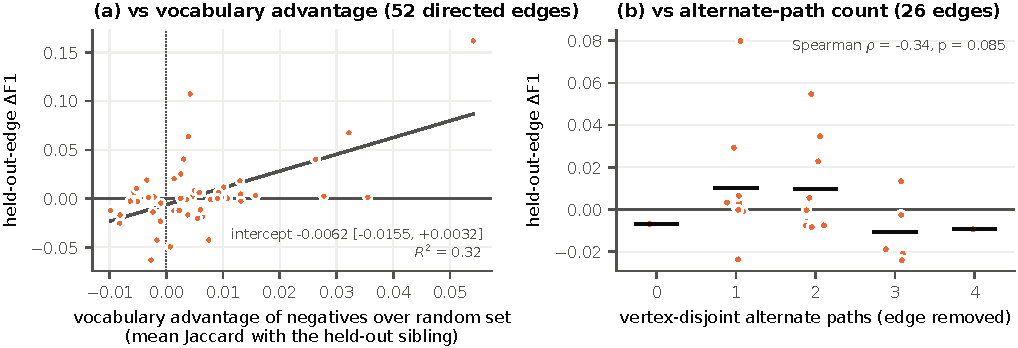
\includegraphics[width=\linewidth]{figures/fig5_per_edge_diagnostics.pdf}
  \caption{Held-out-edge benefit per edge at 70 passages per context (Gemma-2-9B). (a)~Against the vocabulary
  advantage of the held-out-edge negatives over the random negatives; line: OLS fit, whose intercept is the
  vocabulary-adjusted effect. (b)~Against the number of vertex-disjoint alternate paths between the edge's
  endpoints once the edge is removed (undirected edges; bars are group means). Both analyses are exploratory.}
  \label{fig:peredge}
\end{figure}

\section{Concepts}
\label{app:concepts}

\begin{table}[h]
  \centering
  \small
  \caption{SET~G concepts and the definitions recorded in the contrastive boundary graph.}
  \begin{tabular}{p{0.37\linewidth}p{0.56\linewidth}}
    \toprule
    Concept & Definition \\
    \midrule
    \texttt{ManipulativeCommunication} & Communication that steers another party by exploiting framing, pressure, asymmetry, or vulnerability rather than preserving their independent evaluation. \\
    \texttt{PersuasiveCommunication} & Legitimate influence that offers reasons, evidence, or appeals while leaving the recipient's evaluative agency intact. \\
    \texttt{Propaganda} & Systematic messaging that promotes an ideology, group, or agenda by repetition, selective framing, identity pressure, or suppression of contrary context. \\
    \texttt{Misinformation} & False or misleading information spread without the defining feature of deliberate deceptive intent. \\
    \texttt{Disinformation} & False or misleading information spread with deliberate deceptive intent. \\
    \texttt{PsychologicalExploitation} & Use of another party's cognitive, emotional, social, or situational vulnerabilities to steer their beliefs or choices. \\
    \texttt{SycophancyRegister} & A sustained servile or over-agreeable communicative register oriented around pleasing, flattering, or appeasing the recipient. \\
    \texttt{UnwarrantedPraise} & A discrete act of praise that is unsupported, exaggerated, or strategically insincere. \\
    \texttt{ExcessiveAgreement} & Over-agreement with a person's claims, preferences, or judgments beyond what evidence or independent evaluation warrants. \\
    \texttt{Misdirection} & A tactic that redirects attention, salience, or interpretation away from a relevant fact or issue. \\
    \texttt{StrategicDeceptionPlanningProcess} & Planning or sequencing deceptive actions over time to achieve a goal. \\
    \texttt{SpecificationGamingProcess} & Optimizing for a specified metric, rule, or reward in a way that violates the intended objective. \\
    \texttt{UlteriorMotiveDetection} & Detection or inference of hidden motives behind another party's behaviour or communication. \\
    \texttt{Deepfake} & Synthetic or manipulated media depicting a person, event, or signal in a way that can be mistaken for authentic media. \\
    \texttt{Threaten} & An explicit or implied conditional commitment to cause harm, penalty, or loss unless the target complies. \\
    \bottomrule
  \end{tabular}
\end{table}

\end{document}
